\documentclass[11pt, oneside]{article}   	% use "amsart" instead of "article" for AMSLaTeX format
\usepackage{geometry}                		% See geometry.pdf to learn the layout options. There are lots.
\geometry{letterpaper}                   		% ... or a4paper or a5paper or ... 
%\geometry{landscape}                		% Activate for rotated page geometry
\usepackage[parfill]{parskip}    			% Activate to begin paragraphs with an empty line rather than an indent
\usepackage{graphicx}				% Use pdf, png, jpg, or eps§ with pdflatex; use eps in DVI mode
								% TeX will automatically convert eps --1 pdf in pdflatex		
\usepackage{bbm}
\usepackage{amssymb,amsmath,amsthm,bm,pgfplots, xcolor}
\usepackage{mathtools}
\usepackage[style=apa, backend=biber]{biblatex}
\addbibresource{reference.bib}
\usepackage{enumitem}
\usepackage{hyperref}
\usepackage{comment}

\usetikzlibrary{arrows}


\newcommand{\E}[1]{\mathbb{E}\left[#1\right]}



\newenvironment{Solution}[1][Sol]{%
  \begin{proof}[#1]$ $\par\nobreak\ignorespaces
	\qquad
}{%
  \end{proof}
}



\title{Data Science and Social Inquiry: HW3}
\author{Yu-Chang Chen and Ming-Jen Lin}
\date{\today}					

\begin{document}

\maketitle
\section*{Question 1: K-means clustering by hand}

\begin{enumerate}[label = (\emph{\alph*})]
	\item (1 pt) \label{a} What is the optimal clustering that minimizes the
	      total within-cluster sum of squared Euclidean distance?

	      \begin{Solution}
          If $(0,4)\in C_{1}$ and  $(0,0),(3,0)\in C_{2}$:\\
          $\sum_{k=1}^2 \sum_{i\in C_{k}}\sum_{j=1}^2(x_{ij}-\Bar{x}_{kj})^2=(0-1.5)^2+(3-1.5)^2=4.5$\\\\
          If $(3,0)\in C_{1}$ and  $(0,0),(0,4)\in C_{2}$:\\
          $\sum_{k=1}^2 \sum_{i\in C_{k}}\sum_{j=1}^2(x_{ij}-\Bar{x}_{kj})^2=(0-2)^2+(4-2)^2=8$\\\\
          If $(0,0)\in C_{1}$ and  $(3,0),(0,4)\in C_{2}$:\\
          $\sum_{k=1}^2 \sum_{i\in C_{k}}\sum{j=1}^2(x_{ij}-\Bar{x}_{kj})^2=\sqrt{(3-1.5)^2+(0-2)^2}+\sqrt{(0-1.5)^2+(4-2)^2}=12.5$
          
          Hence, the optimal clustering is with the initial cluster assignments$(0,4)\in C_{1}$ and  $(0,0),(3,0)\in C_{2}$
          
	      \end{Solution}
	\item (1 pt)
	      What would be the clustering the algorithm converges to? Is it the
	      same as what you found in part \ref{a}?


	      \begin{Solution}
            
            $\bar{x_{1}}=(0,2)\bar{x_{2}}=(3,0)$\\
            
            $d(x_{1},\bar{x_{1}})=2, d(x_{1},\bar{x_{2}})=3$\\
            $d(x_{2},\bar{x_{1}})=$\sqrt{13}$ d(x_{2},\bar{x_{2}})=0$\\
            $d(x_{3},\bar{x_{1}})=2, d(x_{3},\bar{x_{2}})=5$\\
            
            Hence, $(0,0),(0,4)\in C_{1}$ and  $(3,0)\in C_{2}$ converge
            
            It is not the same as what we found in part (a).




	      \end{Solution}
	\item (1 pt) What is the probability of converging to the global optimum if we run the algorithm again with random initial assignments?

	      \begin{Solution}
            
            \item  If we run the algorithm again with $(0,4)\in C_{1}$ and  $(0,0),(3,0)\in C_{2}$, it converges to the optimal clustering. (part (a))
            
            \item  If we run the algorithm again with $(3,0)\in C_{1}$ and  $(0,0),(0,4)\in C_{2}$, it converges to $(3,0)\in C_{1}$ and  $(0,0),(0,4)\in C_{2}$. (part (b))
            
            \item  If we run the algorithm again with $(0,0)\in C_{1}$ and  $(3,0),(0,4)\in C_{2}$, it converges to $(0,0)\in C_{1}$ and  $(3,0),(0,4)\in C_{2}$.(below)
            
            $\bar{x_{1}}=(0,0)\bar{x_{2}}=(1.5,2)$\\
            
            $d(x_{1},\bar{x_{1}})=0, d(x_{1},\bar{x_{2}})=\frac{1}{2}\sqrt{5}$\\
            $d(x_{2},\bar{x_{1}})=3, d(x_{2},\bar{x_{2}})=1.5$\\
            $d(x_{3},\bar{x_{1}})=4, d(x_{3},\bar{x_{2}})=1.5$\\
            
            Hence, the probability of converging to the global optimum is $\frac{1}{3}$if we run the algorithm again with random initial assignments.
            
            
            
            
            
	      \end{Solution}
\end{enumerate}


\newpage

\section*{Question 2: Selection and shrinkage}

\begin{enumerate}[resume*]
	\item (1 pt) What is the OLS estimate?
	      \begin{Solution}

            $\hat{\beta_{1}}=\frac{1+3}{1+1}=2\\\\
\hat{\beta_{2}}=\frac{2+2+5}{1+1+1}=3\\\\
\hat{\beta_{3}}=\frac{5+3}{1+1}=4\\\\
\hat{\beta_{4}}=\frac{4+6+5}{1+1+1}=5\\\\$

Hence, the fitted value of $y$ by OLS method is $\hat{y}=2x_{1}+3x_{2}+4x_{3}+5x_{4}$




	      \end{Solution}
	\item (1 pt) What is the LASSO estimate with penalty term $\lambda=12$?
	      \begin{Solution}
            $\min\sum_{i=1}^{10}(y_{i}-\beta_{1}x_{1}-\beta_{2}x_{2}-\beta_{3}x_{3}-\beta_{4}x_{4})^2+\lambda\sum_{j=1}^{10}|\beta_{j}|\\\\
            2\sum_{i=1}^{10}(y_{i}x_{i}-\beta x_{i}^2)-\lambda=0\\\\
            \hat{\beta_{1}}=\frac{2\sum_{i=1}^{10}(x_{i}y_{i})-\lambda}{2\sum_{i=1}^{10}(x_{i}^2)}\\\\
            2<\sqrt{12}{4}  \Rightarrow \beta_{1}=0\\\\
            \beta_{2}=3-\sqrt{12}{6}=1\\\\
            \beta_{3}=4-\sqrt{12}{4}=1\\\\
            \beta_{4}=5-\sqrt{12}{6}=3\\\\$

Hence, the LASSO estimator with penalty term $\lambda=12$  is $y=x_{2}+x_{3}+3x_{4}+\epsilon$
	      \end{Solution}
	\item (1 pt) How does the size of the penalty term affect our LASSO estimate?
	      Plot the LASSO estimates $(\hat{\beta}_1^{L}, \hat{\beta}_2^{L}, \hat{\beta}_3^{L},
		      \hat{\beta}_4^{L})$ as functions of $\lambda\in[0,50]$.
	      \begin{Solution}
		      %Try using PgfPlots:)
		      %To plot conditional functions, one could write the function using the ternary operator <if> ? <then> : <else> in one line.
		      %Modify the following code to obtain the desired plot.

		      \begin{center}
			      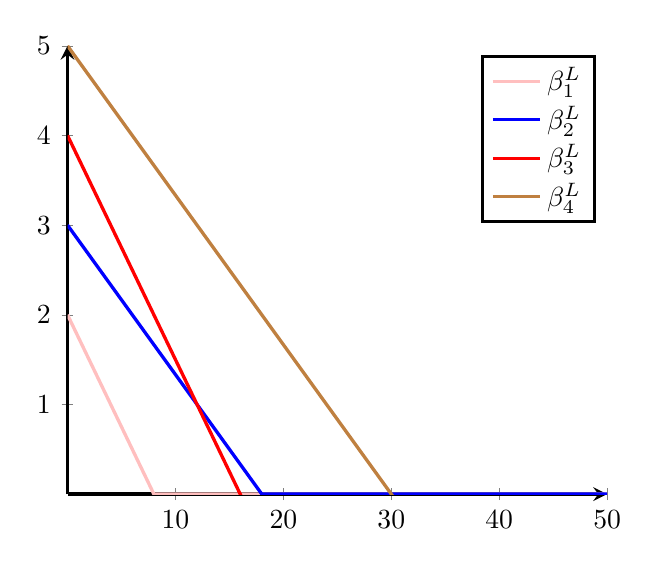
\begin{tikzpicture}
				      \begin{axis}[
						      axis lines = middle,
						      xmin = 0, xmax = 50,
						      ymin = 0,
						      very thick,
						      legend entries = {$\beta_1^L$, $\beta_2^L$, $\beta_3^L$, $\beta_4^L$},
					      ]
					      \addplot[domain=0:50, samples=201, pink] {2-x/4 > 0 ? 2-x/(2*2) : 0};
					      \addplot[domain=0:50, samples=201, blue] {3-x/6>0 ? 3-x/6 : 0};
					      \addplot[domain=0:50, samples=201, red] {4-x/4 ? 4-x/4 : 0};
					      \addplot[domain=0:50, samples=201, brown] {5-x/6 ? 5-x/6 : 0};
				      \end{axis}
			      \end{tikzpicture}
		      \end{center}

		      %There are lots of options can be customized. Read pgfplots manual for more information.
	      \end{Solution}



	\item (1 pt) Compare the three estimates you found. Can you see where
	      the name ``Least absolute and Shrinkage and Selection Operator''
	      comes from?
	      \begin{Solution}
We can see that when $\lambda$ gets larger, the more coefficients will be selected and shrink to 0. Only the ones who have larger average will be selected. In this case, when $\lambda$ is larger or equal to 8,16,18,and 30 separately, $\beta_1^L$, $\beta_3^L$, $\beta_2^L$, and $\beta_4^L$ will sequentially shrink to zero as well.
	      \end{Solution}
\end{enumerate}

\newpage

\section*{Question 3: Predict stock returns with LASSO}
\begin{enumerate}[resume*]
	\item (1 pt) How many parameters (including the intercept) are we estimating?
	      \begin{Solution}
            There are 3,067 companies,three periods (t = 3) and an intercept , which means there are 9,202 parameters.  
	      \end{Solution}
	\item (1 pt) Use the five-fold cross-validation to select the optimal penalty
	      term $\lambda$. What is the optimal $\lambda$ you find?
	      \begin{Solution}
                The optimal $\lambda$ we found was 0.000046.
	      \end{Solution}
	\item (1 pt) Use the $lambda$ you found to estimate the coefficients.
	      How many coefficients are non-zero? What are the stocks with
	      non-zero coefficients?
	      \begin{Solution}
            With $\lambda$ equals 0.000046, there are 23 non-zero 
            coefficients.\\
                The companies are : \\ \\
                BAC($t_1$), BRK($t_1$), IVR($t_1$), LTRP($t_1$), NGL($t_1$), SMMC($t_1$)\\ \\
                UONE($t_1$), WPG($t_1$), BAC($t_2$), BRK($t_2$), OPES($t_2$), SMMC($t_2$)\\ \\
                WFC($t_2$), BAC($t_3$), BRK($t_3$), CLNY($t_3$), GLOG($t_3$), GLOP($t_3$)\\ \\ NYMT($t_3$),
                PEI($t_3$), QRTE($t_3$), TWO($t_3$), WFC($t_3$).
            
	      \end{Solution}
\end{enumerate}
\end{document}

